\section{Related Work}
\label{s:related-work}


Search Enginee Optimization (SEO) is encouraged by Seach Enginee companies like Google to improve the indexing and searching accuracy. SEO technology being used should follow the Google Policy. However, because imfluencing the search results has huge commerical incentives, some hackers designed Black Hat SEO which violate Google's policy. Cloaking is a representative of Black Hat SEO. Websites feed different information between Google and Users. In our study, we found that cloaking not only exists in SEO field but also Search Engiee Marketing (SEM). SEM is a term that exclusively to mean pay per click advertising, particularly in the commercial advertising and markerting communities which have a vested interest in thisnarrow defination. Advertisers pay Google to advertise one kind of advertisements. By cloaking, advertisers actually cheat Google and provide different kinds of advertisements, even maladvertising~\cite{Li:2012:KYE:2382196.2382267} and malicious attacks. 

\subsection{Cloaking Example}
To see the bad reputation of cloaking, we give two examples: malicious download cloaking and advertisement cloaking. As an example of malicious download cloaking, enter the term "Game Texas Holdem Poker Online - Dj W" in Google, return a set of search results as showned in figure 1.
The top 6 search results are all under domain "djw.com.pl" and cloaking websites. If we disguised ourselves as normal users without setting HTTP proxy agent and clicked the links, the HTTP request 
to these websites included an Google Signature. These cloaking websites detected this Google Signature and redirected serveral times to an landing page with malicious automatic downloads. Then we 
typed the website URL directly to the brower or set the HTTP proxy as Google-bot. We revisited the website and saw different content without malicious downloads. The cloaking idea is clear. To avoid Google censorship system find their maclicious downloads, the websites serves benign content related to "Game Texas Holdm Poker Online" if visits are from Google IP address or directly input url. Because this website is a unknown small website, most of their visits are from Google Search. Thus, the website only show their mailicious downloads when visits are from Google search results while serve benign content to direct URL access and Google IP address. 
As an example of advertisement cloaking, enter the term "essay writing" on Google on Feb 6, 2015 returned a set of search results and advertisements related to essay writing. (The appendix includes screenshots of this example.) For the second advertisement result in right side, the bold line circle the webstie (everlastinghelp.com) that sent "Homework assignment help" to users when users click the link from Google. After we set our browser agent as Google-bot, we accessed the same website again. This time, the website sent totally different content about travel to us. In this example, homework assignment help is classified as dishonest behaviors which is not allowed by Google-Ads-Words Policy. To get profits by providing illegal services and survive from the cencorship of Google, this website (everlastinghelp.com) identify Google-bots by IP address and serve Goolge-bots different content  from users. 
From these two examples, we see different incentives of cloaking. In first example, the incentive of cloaking is malicious downloading. In second example, the incentive of cloaking is providing 
illegale serices. To understand various cloaking incentives, we will introcuce areas such as search enginee optimization(SEO) and search enginee marketing(SEM) where enourmous cloaking exists. To understand 
mechamisms of cloaking, we will introduce types of cloaking such as IP cloaking, referrer cloaking, repeat cloaking and user-agent cloaking. 


\begin{figure}[t]
	\centering
	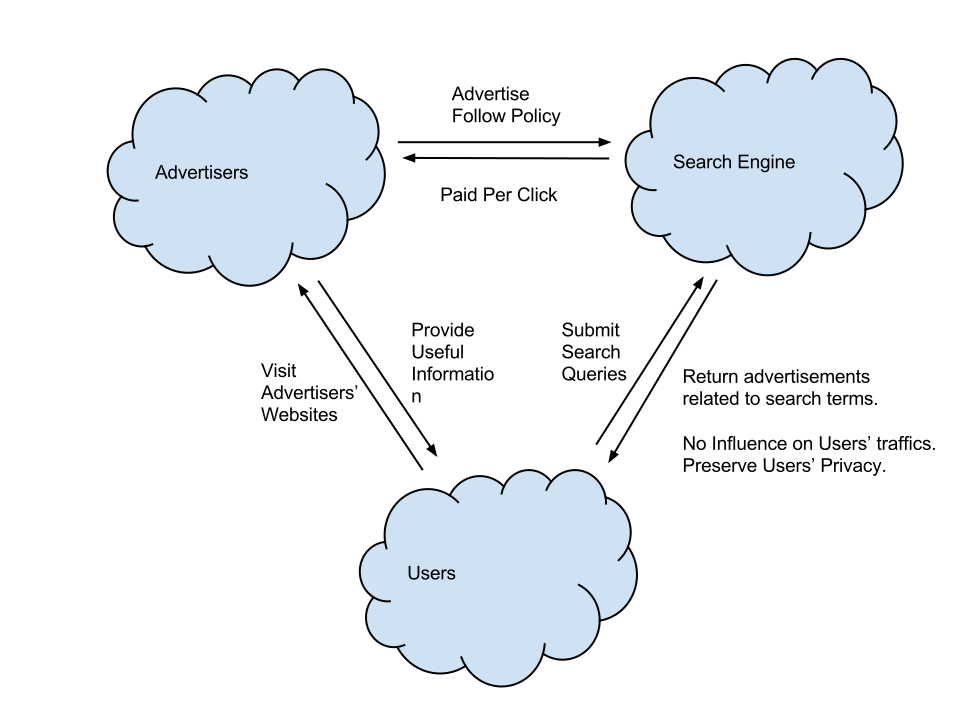
\includegraphics[width=.5\textwidth]{fig/three-parties}
	\label{fig:sem-model}
	\caption{Three-paries relationships in SEM}
\end{figure}

\subsection{Cloaking Detection}
Talk about cloaking detection related work here.
According to ~\cite{wang2011cloak}, they used the precision rate to measure the cloaking distribution on the search enginee hot terms. However, precision is highly depends on TRP and FPR. Using the precision to measure the distribution is fundamentally wrong method to do that. One of the right ways is using the TPR and FPR to measure the distribution. Another mistake they made is using constant numbers to measure time-based data without doing cross-validation. One way to do that is using the cross-validation or time-based adaptive parameter to solve this problem. 

Tree party relationships in SEM field. 
To better understanding the advantages of our crowdsourcing model, we briefly introduce the relationships in Search Enginee Marketing (SEM). In Search Enginee Marketing, there are thhree parties: Search Engine Providers, Advertisers and Users. Advertisers post their advertisements on the search enginee ads lists. Search engines are paid when the advertisements are clicked. While the advertisements are posted on the search enginee, they must obey the search enginee advertisements policy. In Google AdWords policies~\cite{google-ads-policy}, there are four types of policies: Prohibited content, Prohibited practices, Restricted content, Editoral and technical. Prohibited content indicates that content that not allowed to apromote on the Google Network, i.e., conterfeit or dangerous products. Prohibited practices means that things advertisers can't do, i.e., malicious ads, sites or apps. Restrided content that there are limitations on content, i.e., Adult-oriented content, Alcoholic beverages or Gambling-related content. Editorail\&technical requirements indicate ads should be engaging for users without being annoying or difficult to interact with, i.e., gimmicky use of words, numbers, letters, punctuation or symbols such as FREE, f-r-e-e, and F₹€€!!. When users submit search terms on the search enginees, search enginees provide users ads that related to their search terms. Attractive ads are clicked by users. That's how advertisers promote their products and search enginees like Google get paid. 

In order to sell products or services that don't follow the Search Enginee Policy and get profits, advertisers cheat Google by cloaking. Advertisers send the content that follow the Google Policy to Google while serve a totally different contant that break the Google policy to users. Cloaking detection methods proposed by ~\cite{wang2011cloak} couldn't 

Traditional cloaking detection model only targets SEO field, our simhash based cloaking detection method could work both on SEO and SEM field. The main difference between the SEM and SEO is that every link in SEM is "pay per click". This indicates that  traiditional crawler will increase the advertisers payments by clicking the search result links and collecting data. If the cralwers first collect the landing page of the search result links then visit urls to collect data. The crawlers won't find the referal cloaking accoding to defination of referal cloaking. However, in our crowdsoucing model, the data we collected is from real users' clicks. Advertisers wouldn't pay extra money because of data collection. 
Model based on crowdsourcing could preserve the three party relationships between Users, Search Enginee Providers and Advertisers.

why cloaking matters in security field?
malicious download, illegal drugs, illegal services, guns, phishing site, 



1.David Y. Wang Single IP not efficient in  IP cloaking.
2.text shingling computation complexity is o(nlgn), simhash is 0(n). 5 bilion pages are indexed by google. 
2.While David Y. Wang crawlers disguised as users, crawlwers are still not users. There is no proof whehter the data collected by cralwer disguised as users could is exact same aas user sees. 
2.5 David Y. Wang crawlers are actively crawl data. We are passively receive the SimHash Value compare. 
3.distributed workload computation--distributed the part of computation work (SimHash calculation) to users. Servers only needs to compare the SimHash value. David Y. Wang need to do whole computation. 
4.cloaking is dynamic. users could monitor the webstite every time. cralwers could only peredically crawl. But users will give us much more data.
5.map(url1, simhash1)cloaking,  map(url2,simhash2) if simhash2==simhash1, high likely that url2 is cloaking. when a new (url, simhash) come, we firstly index the url. if simhash match, highly possible
cloaking. If not same, then compute the existed one. Index a simhash value only takes o(1) time. If we compare, this will takes google crawl 6 times, compute a simhash model and compare the user 
simhash value and simhash model. it takes too much time. Many cloaking websites are shareing the same content. show figure. \XXX{} building this simhash table takes 2^64. It's enought to measure 
cloaking websites because the whole websites is 5 billion(2^34) which is also dynamic. simhash table (simhash value, cloaking or not or percentages of cloaking websites in this field). Using the traditional one, they couldn't find this. They firstly need to store the whole cloaking websites. Not enought storage. Then indexed a same cloaking website. Indexing cost is higher than O(1). 
6. Our simhash model mearsue time is smaller than most of cloaking changing duration. Wouldn't miss any cloaking because cloaking change too slowly. Traditional crawleing would miss. 
\subsection{Simhash}
Talk about simhash related work here. \\
Simhash~\cite{charikar2002similarity}  is a locality sensitive hash algorithm.
It is widely used by search engine to detect near duplicate of websites.


Show what simhash does and how they are used in the past.

Some embedded literal typeset code might 
look like the following :

{\tt \small
  \begin{verbatim}
  int wrap_fact(ClientData clientData,
  Tcl_Interp *interp,
  int argc, char *argv[) {
    int result;
    int arg0;
    if (argc != 2) {
      interp->result = ``wrong # args'';
      return TCL_ERROR;
    }
    arg0 = atoi(argv[1]);
    result = fact(arg0);
    sprintf(interp->result,``%d'',result);
    return TCL_OK;
  }
  \end{verbatim}
}

Now we're going to cite somebody.  Watch
for the cite tag.
Here it comes%~\cite{Chaum1981,Diffie1976}.
The tilde character (\~{})
in the source means a non-breaking space.
This way, your reference will
always be attached to the word that preceded it,
instead of going to the
next line.


\subsection{Simhash in Cloaking Detection}
Show the story here please!

1.what is the technical challege that we are addressing? compared to traditional
methods.

a. attacker could incrementally block inspector IP
b. crowdsourcing is cheap, compared to buying new IPs
c. crowdsourcing match user distribution and user habbit on web ~\cite{wang2011cloak}.

2. why we need simhash.
reduce volume of data, and collect enough information for cloaking detection.


3. what is user incentive?
build an extension to help user understand whether this website is
safe/compliant or tricking user by cloaking

user privacy is protected and can get better service.




